% Chapter 1

\chapter{Desarrollo} % Main chapter title

\label{Chapter1} % For referencing the chapter elsewhere, use \ref{Chapter1} 
\label{IntroGeneral}

%----------------------------------------------------------------------------------------

% Define some commands to keep the formatting separated from the content 
\newcommand{\keyword}[1]{\textbf{#1}}
\newcommand{\tabhead}[1]{\textbf{#1}}
\newcommand{\code}[1]{\texttt{#1}}
\newcommand{\file}[1]{\texttt{\bfseries#1}}
\newcommand{\option}[1]{\texttt{\itshape#1}}
\newcommand{\grados}{$^{\circ}$}

%----------------------------------------------------------------------------------------

%\section{Introducción}

%----------------------------------------------------------------------------------------
\section{Introducción}

En el presente trabajo práctico se desarrolla, como una continuación del trabajo práctico 1, la implementación del algoritmo \textit{Proximal Policy Optimization} (PPO) en el juego de Tetris, evaluándolo y comparándolo con los algoritmos DQN y Dueling-DQN ya presentados.

Para lograrlo, se adaptó el ambiente de Tetris del trabajo anterior, creando una nueva clase \textit{TetrisGymWrapper} que extiende el ambiente \textit{gym} de \textit{gymnasium}. Esta extensión permite utilizar la librería \textit{stable\_baselines3} que posee implementados algoritmos avanzados de aprendizaje por refuerzo y métodos de entrenamiento fáciles de utilizar. En la sección \ref{sec:entorno} se comentan más detalles del ambiente.

Para el agente, se utilizó la clase \textit{PPO} de la librería \textit{stable\_baselines3} mencionada. En la sección \ref{sec:agente} se describe el mismo con mayor detalle.

Finalmente, se realizaron también modificaciones al script principal main.py para adaptarlo a la ejecución de los casos de uso principales (entrenar el modelo y ejecutarlo sobre un ambiente visual) teniendo en cuenta los requerimientos de interfaz de las librerías utilizadas.

\section{Entorno}
\label{sec:entorno}

El juego comienza luego instanciar la clase \textit{GameUI} y ejecutar el método \textit{play}. Esta clase administra la interfaz gráfica del juego de Tetris utilizando la librería \textit{pygame}, y también administra la interconexión con la librería \textit{gymnasium} utilizando la clase \textit{TetrisGymWrapper} sobre el juego de Tetris. 

\textit{TetrisGymWrapper} extiende de \textit{gym} y sobreescribe los métodos \textit{init}, donde inicializa el juego de Tetris subyacente, \textit{reset} para reiniciar el juego, y \textit{step} para ejecutar una acción dada como parámetro sobre el ambiente y retornar la terna [nuevo estado, recompensa, juego finalizado].

Al utilizarse de trasfondo la misma clase de juego de Tetris que en el trabajo anterior, los detalles del ambiente se repiten: 
\begin{itemize}
    \item El juego imprime en pantalla el tablero de la figura \ref{fig:board}. 
    \item Se permiten 5 acciones: abajo, derecha, izquierda, rotar y omitir.
    \item El estado observado del ambiente consta de una matriz de 20 filas y 10 columnas (tamaño del tablero de Tetris), donde cada elemento de la matriz es 255 si la posición respectiva en el tablero está ocupada por un bloque (ya sea el bloque actual o uno fijado) o 0 si la posición está libre. La razón de utilizar 255 es que de esta manera PPO interpretará a la matriz como una imagen blanco y negro del tablero.
\end{itemize}

\begin{figure}[htbp]
	\centering
	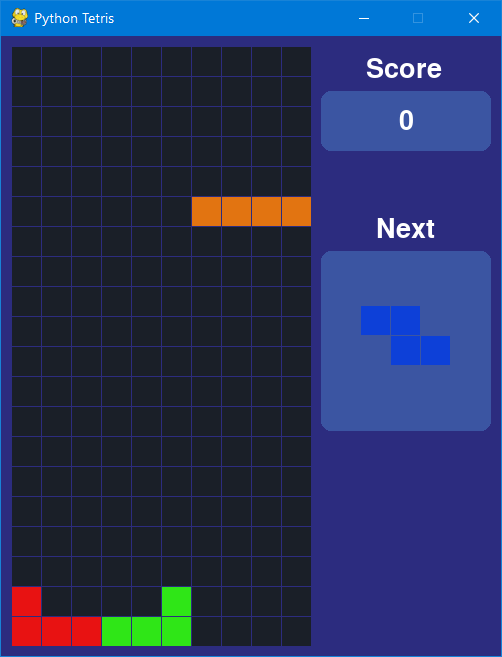
\includegraphics[width=.5\textwidth]{./Figures/tetris.png}
	\caption{Tablero de Tetris.}
	\label{fig:board}
\end{figure}

Para los puntajes, se comenzó con el esquema anterior de asignar 1 punto por cada ejecución de la acción abajo, 100 puntos por completar una línea, 300 por completar 2 líneas en simultáneo y 500 por completar 3. Se observó que esta función no daba buenos resultados, por lo que se realizaron modificaciones que se comentan en la sección \ref{sec:entrenamiento}.

\section{Agente}
\label{sec:agente}

Por simplicidad, en este caso el juego admite como jugadores solamente modelos de la librería \textit{stable\_baselines3}. Estos se encuentran restringidos a ejecutar un solo movimiento cada 200 ms. Es decir, en cada turno (cada 200 ms) el modelo observa el estado actual del tablero como una imagen blanco y negro, se toma una de las 5 acciones posibles según la política aprendida, el ambiente se actualiza ejecutando la acción y luego moviendo el bloque actual una posición hacia abajo.

Para la arquitectura de red neuronal del agente, se decidió continuar en base a los resultados obtenidos en el trabajo anterior y se utilizó PPO con política \textit{CnnPolicy}, que permite interpretar al tablero como una imágen. En la figura \ref{fig:arquitectura} se presenta la arquitectura extraída de los documentos de la librería \textit{stable\_baselines3}, donde el denominado \textit{feature extractor} para este caso esta formado por una red CNN de 3 capas con 32, 64 y 64 filtros respectivamente.

\clearpage

\begin{figure}[hbt!]
	\centering
	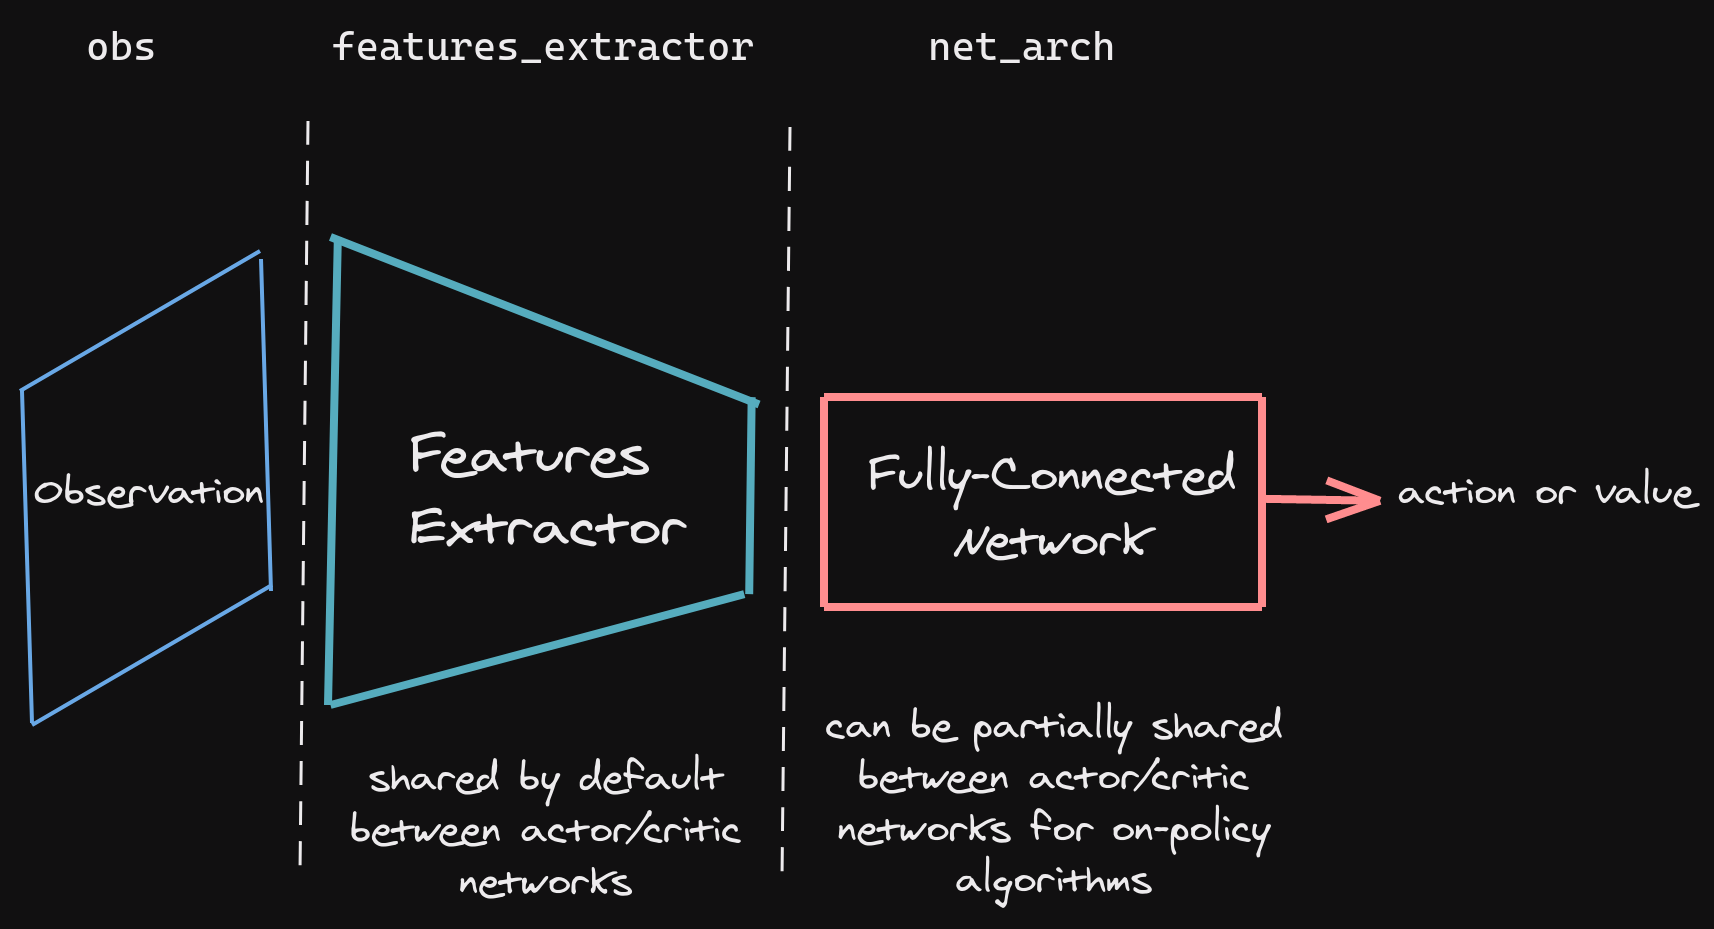
\includegraphics[width=\textwidth]{./Figures/architecture.png}
	\caption{Arquitectura PPO.}
	\label{fig:arquitectura}
\end{figure}

\section{Entrenamiento}
\label{sec:entrenamiento}

Para entrenar el agente de PPO, se ejecutaron múltiples juegos consecutivos de Tetris con la participación del modelo en entrenamiento y sin impresión de la interfaz gráfica. 

Dentro de una nueva clase creada llamada \textit{TrainerPPO} se ejecutó el método \textit{make\_vec\_env} de \textit{stable\_baselines3}, especificando como parámetro la clase \textit{TetrisGymWrapper}, para crear un ambiente personalizado de \textit{gymnasium} listo para ser utilizado con cualquier algoritmo de la librería. Luego se creó una instancia de la clase PPO y se llamó al método \textit{learn} para ejecutar el entrenamiento sobre el ambiente creado en el paso anterior. Adicionalmente, en el método \textit{learn} se especificaron 2 métodos \textit{callback} que permiten guardar los modelos intermedios cada 100.000 pasos y registrar los retornos obtenidos en cada episodio del juego. En total el entrenamiento se ejecutó por 10.000.000 pasos, equivalente a aproximadamente 60.000 episodios. Este entrenamiento demoró 21 horas.

En el primer experimento de entrenamiento se utilizó el sistema de recompensas del trabajo anterior. Se observó que los resultados obtenidos con este algoritmo eran pobres, ya que llevabnan al agente a simplemente ejecutar la acción abajo para bajar los bloques lo más rápido posible y obtener la pequeña recompensa de esta acción. Luego de investigar, se encontraron las publicaciones \citep{ARTICLE:1} y \citep{ARTICLE:2} donde se sugieren nuevos algoritmos de recompensa.

\citep{ARTICLE:1} propone la fórmula:
\begin{equation}
    0.7*CompleteLines-0.5*AggregateHeight-0.3*Holes-0.2*Bumpiness
\end{equation}

Donde \(CompleteLines\) es la cantidad de líneas completas, \(AggregateHeight\) es la suma de las alturas de cada columna del juego, \(Holes\) es la cantidad de espacios sin ocupar que tienen por arriba un bloque ocupado (las posiciones huérfanas de difícil acceso en el tablero) y \(Bumpiness\) es la diferencia en valor absoluto de las alturas de las columnas contiguas. Esta heurística intenta disminuir la altura general de todas las columnas, la cantidad de huecos sin ocupar y la diferencia de altura entre las columnas.

\citep{ARTICLE:2} propone una heurística más simple, dada por la fórmula:
\begin{equation}
    A*CompleteLines-B*MaxHeight-C*Holes
\end{equation}

Donde \(MaxHeight\) es la altura máxima alcanzada y \(CompleteLines\) y \(Holes\) comparten significado con el caso anterior.

Al implementar ambos, se observó que \citep{ARTICLE:2} obtuvo mejores resultados. Los pesos para cada componente se ajustaron manualmente mediante sucesivos experimentos, obteniendo:
\begin{equation}
    A=0.7 \quad B=0.5 \quad C=0.3
\end{equation}

\section{Resultados}

Luego de entrenar el agente PPO se obtuvo la curva de recompensa de la figura \ref{fig:ppo_rewards}.

Se observa que la media móvil de la recompensa aumenta lentamente con el paso de los episodios desde un valor de 30 hasta aproximadamente 50, lo que indica que el modelo está entrenándose. Cabe destacar que en este caso bajar bloques no generaba recompensa por lo que el aumento de la media móvil se da mayormente por completar líneas. Si observamos la evolución de la recompensa sin filtrar, notamos que a medida que avanza el entrenamiento la cantidad de veces que se obtienen recompensas mayores a 100 y hasta mayores a 200 son mas frecuentes..

\begin{figure}[htbp]
	\centering
	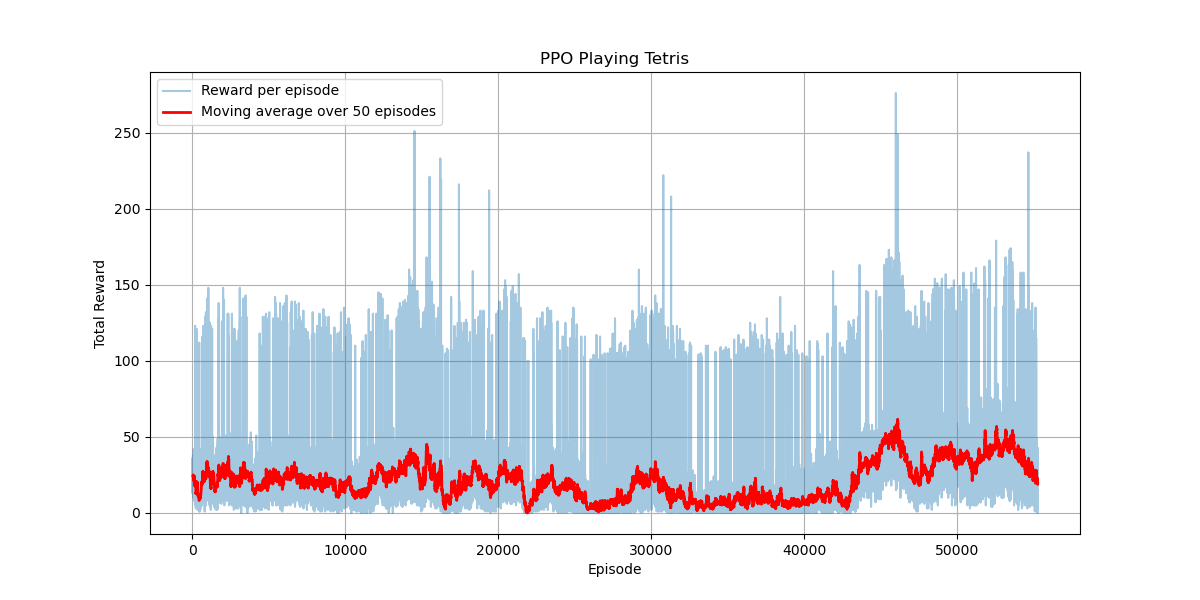
\includegraphics[width=\textwidth]{./Figures/ppo_rewards.png}
	\caption{Recompensa por episodio para algoritmo de PPO, suavizado con una media móvil de 50 episodios.}
	\label{fig:ppo_rewards}
\end{figure}

Al ejecutar el juego con el modelo entrenado como jugador, se observa que intenta completar lo máximo posible la grilla moviendo y rotando las piezas. Realiza una distribución a lo ancho del tablero, intentando tapar los huecos huérfanos cuando es posible y eventualmente completando 1 o hasta 2 líneas.

\begin{figure}[htbp]
	\centering
	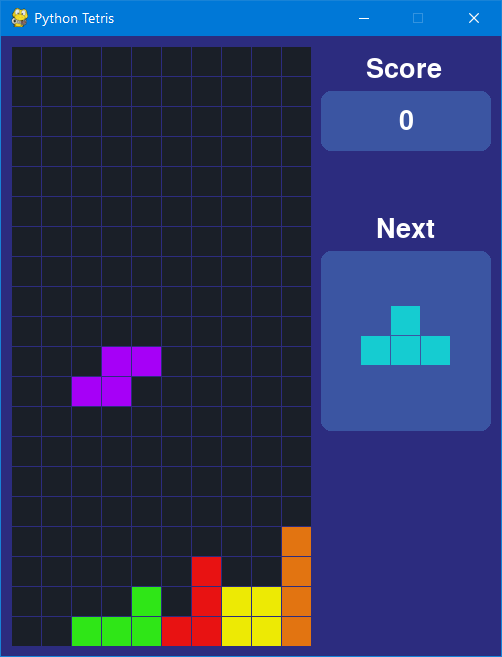
\includegraphics[width=0.5\textwidth]{./Figures/ppo_playing.png}
	\caption{Agente Double-DQN distribuyendo bloques a lo ancho del tablero.}
	\label{fig:ppo_playing}
\end{figure}

\section{Conclusiones}
\label{sec:conclusions}

PPO demostró resultados satisfactorios, aprendiendo a distribuir bloques a lo ancho del tablero, llenando los denominados huecos huérfanos y completando ocasionalmente líneas. Si bien los resultados no son ideales, las mejoras respecto a los algoritmos de DDQN y Dueling-DQN probados en el trabajo anterior son notorias. Adicionalmente, el costo de codificar el modelo y el ambiente en este caso fue en gran medida menor que en los algoritmos del trabajo anterior gracias a la utilización de las librerias \textit{gymnasium} y \textit{stable\_baselines3}.

\section{Trabajo futuro}

Como trabajo futuro se plantea investigar otras fórmulas de recompensa que obtengan mejores resultados (que completen mayor cantidad de lineas en forma consistente), como las recopiladas en \citep{ARTICLE:3}; y estudiar otras posibles codificaciones de las observaciones del entorno u otro espacio de acciones que simplifiquen el entrenamiento del algoritmo de aprendizaje por refuerzo en el juego de Tetris.